% !TeX spellcheck = it_IT
\documentclass[a4paper,12pt]{article}

\usepackage{alltt, fancyvrb, url}
\usepackage{graphicx}
\usepackage{algorithmic}
\usepackage[utf8]{inputenc}
\usepackage{titling}
\usepackage{fancyhdr}
\usepackage{fontenc}
\usepackage{amsmath,mathtools,algorithm}
\usepackage{amssymb}
\usepackage{longtable}
\usepackage{setspace}
\usepackage{listings}
\usepackage{color}
\usepackage{eurosym}
\usepackage{array}
\usepackage[referable]{threeparttablex}
\usepackage{pifont}

\newcommand{\cmark}{\ding{51}}
\newcommand{\xmark}{\ding{55}}

\usepackage[italian,hidelinks]{hyperref}

\usepackage[italian]{babel}
\usepackage[italian]{cleveref}


\pretitle{%
	\begin{center}
		\LARGE
	}
\posttitle{\end{center}}


\title{\Huge \textbf{Evolutionary Cars} \\
	\vspace{10pt}
	\vspace{20pt}
}
\author{
	Gabriele Graffieti \\ \small \url{gabriele.graffieti@studio.unibo.it}
	\vspace{15pt}
	\\
	Alfredo Maffi \\ \small \url{alfredo.maffi@studio.unibo.it}
	\vspace{15pt}
	\\
	Manuel Peruzzi \\ \small \url{manuel.peruzzi@studio.unibo.it}
}

\date{}

\begin{document}

\maketitle
\pagenumbering{arabic}
\newpage
\tableofcontents
\newpage

\section{Introduzione}

Questo documento è la relazione del progetto Evolutionary Cars, realizzato per il corso di Sistemi Intelligenti Robotici, erogato dalla facoltà di Ingegneria e Scienze Informatiche dell'Università di Bologna (A.A. 2017/2018).

\section{Stato dell'arte}

\section{Architettura}
In questa sezione verrà illustrata l'architettura generale del sistema, rappresentata in \autoref{architecture-diagram}. La progettazione del sistema è stata effettuata in modo da isolare gli aspetti chiave da quelli relativi alla simulazione. Di conseguenza il sistema risulta suddiviso in due sottoparti principali: \emph{core} e simulazione. La parte core raggruppa al suo interno tutti i concetti del sistema che si rivelano indipendenti dall'ambiente nel quale viene eseguito il sistema. D'altro canto, la parte di simulazione si rivela necessario per permettere al sistema di adattarsi ed essere eseguito in un certo ambiente, sia esso reale o virtuale. Segue una breve descrizione dei componenti del sistema.
\begin{description}
	\item[Driver Agent] entità preposta alla guida di un'auto. Indipendentemente dall'implementazione della \emph{Car}, determina la potenza del motore e la direzione di sterzata della stessa, a partire dalle informazioni relative alla distanza dai muri del circuito. Ogni decisione che incide sul movimento dell'auto è determinata da una rete neurale interna, i cui pesi sono regolati in modo da aderire al genotipo dell'agente.
	\item[Neural Network] rete neurale feedforward utilizzata per pilotare un'auto. Riceve in input cinque valori di prossimità, che descrivono lo stato dell'auto in relazione ai muri del circuito, e produce in output forza motore e direzione dello spostamento successivo. I pesi della rete sono inizialmente definiti in modo casuale, per poi essere adattati in corso d'opera in seguito all'evoluzione del genotipo corrispondente.
	\item[Genotype] Insieme di informazioni che contraddistinguono il comportamento di un'auto da un'altra. In particolare, contiene i pesi da assegnare alla \emph{neural network} di un particolare agente.
	\item[Genetic Algorithm] algoritmo finalizzato all'evoluzione dei genotipi da una generazione alla successiva. Si compone delle fasi di selezione, crossover e mutazione, che saranno discusse nel dettaglio in \autoref{evolution}.
	\item[Controller] può essere definito come il collante tra le parti di core e simulazione del sistema. Si occupa inizialmente di istanziare l'algoritmo genetico ed un insieme di driver agent. È responsabile dell'avvio del processo di \emph{evaluation} dei genotipi, interagendo con un componente relativo alla gestione della parte di simulazione. Al termine di tale processo viene notificato, in modo da poter poi provvedere all'avvio della fase di evoluzione, interagendo con l'algoritmo genetico.
\end{description}
In \autoref{architecture-diagram} è illustrato un diagramma che descrive, in maniera informale, l'architettura del sistema. La parte relativa alla simulazione verrà trattata ed approfondita in \autoref{simulation}.

\begin{figure}[H]
	\centering
	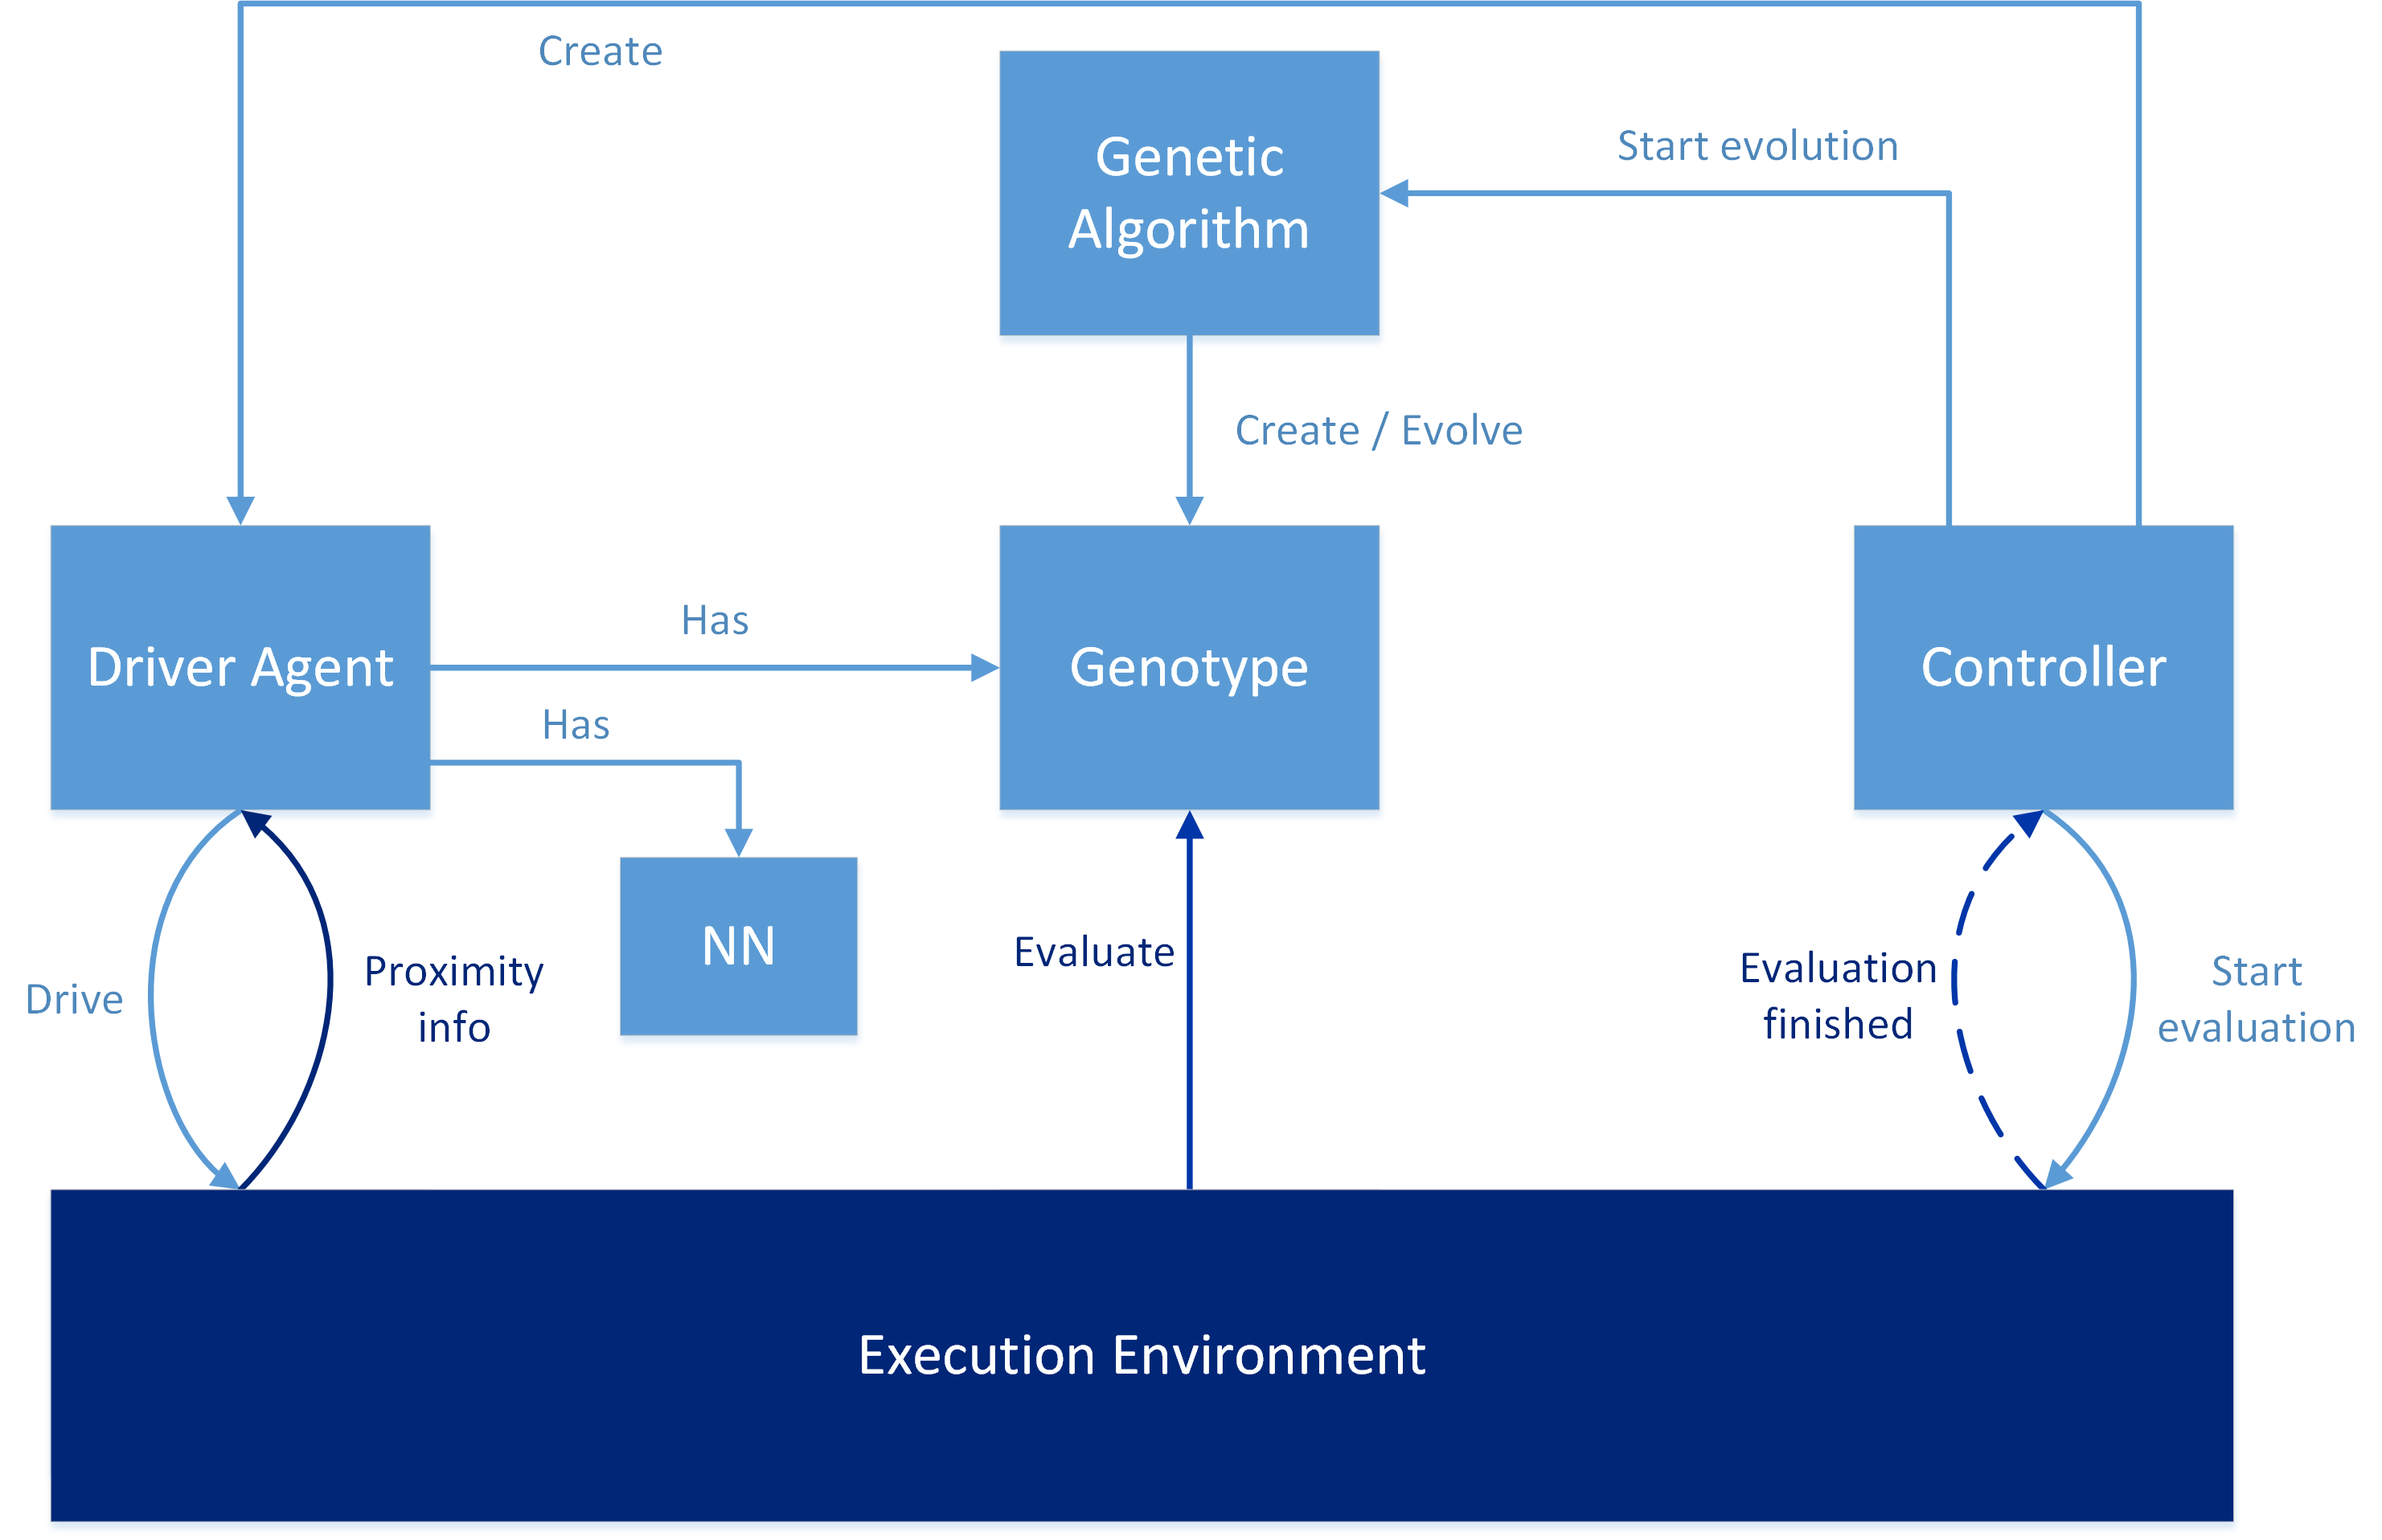
\includegraphics[width=130mm]{./img/architecture.png}
	\caption{Diagramma informale che rappresenta le relazioni tra i componenti che formano l'architettura del sistema. Nella notazione utilizzata, le frecce tratteggiate indicano una notifica dell'avvenimento di un certo evento, a differenza delle frecce continue che si riferiscono a relazioni di dipendenza. Nel diagramma i componenti caratterizzati da un colore più scuro sono quelli relativi alla simulazione, distinguibili dai restanti che costituiscono invece il \emph{core} del sistema.  \label{architecture-diagram}}
\end{figure}

\section{Evoluzione} \label{evolution}

\section{Simulazione} \label{simulation}

\section{Risultati}

\section{Conclusioni}

\end{document}
